\documentclass[tikz, border = 10pt]{standalone}

\usetikzlibrary{positioning, quotes, calc, arrows.meta, shapes}
\renewcommand{\familydefault}{\sfdefault} 
\definecolor{orange}{HTML}{CB6015}

\begin{document}
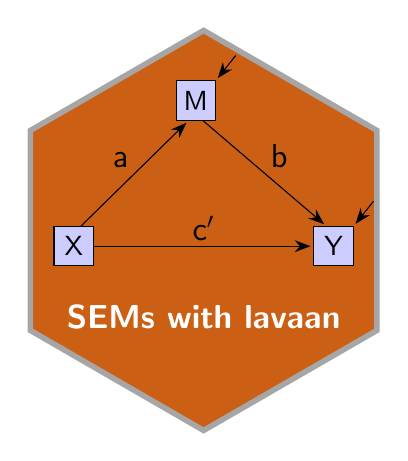
\begin{tikzpicture}

\tikzset{
manifest/.style = {rectangle, draw,  inner sep = 2pt, minimum width = 0.5cm, 
	minimum height = 0.5cm, fill = blue!20},
residual/.style = {rectangle, minimum width = 0.5pt, minimum height = 1.5mm, 
	inner sep = 0pt, outer sep = 0mm},
regression/.style = {-{Stealth[length = 2mm]}, shorten > = 1pt, inner sep = 2pt},
}

%% Hexagon
\node (hexagon) [draw, color = black!35, fill = orange, line width = 2pt, 
   regular polygon, regular polygon sides = 6, rotate = 30, minimum size = 5.08cm] {};

%% SEM
% Manifest
\node at (-1.65, -0.2) [manifest] (X) {X};
\node at (1.65, -0.2) [manifest] (Y) {Y};
\node at (-.1, 1.65) [manifest] (M) {M};

% Regressions
\path [regression] (X) edge ["\large{c$'$}"] (Y);
\path [regression] (X.70) edge ["\large{a}"] (M.250);
\path [regression] (M.290) edge ["\large{b}"] (Y.110);

% Residuals
\node [residual] (e2) [above right = 2.5mm and 2.5mm of Y] {};
\node [residual] (e1) [above right = 2.5mm and 2.5mm of M] {};
\path [regression] (e2) edge (Y.north east);
\path [regression] (e1) edge (M.north east);

%% Label
\draw (0, -1.1) node [text = white] {\bf\large{SEMs with lavaan}};

\end{tikzpicture}
\end{document}